% inhaltlich  vollständig 
% todo: Redigieren

\chapter{Konzeptuelle Einordnung} % (fold)
\label{cha:konzeptuelle_evaluierung}

An dieser Stelle erfolgt ein Rückgriff auf die in Abschnitt \ref{sec:konzeptualisierungen_von_tangible_interfaces} beschriebenen konzeptuellen Beschreibungs-Ansätze für Tangible User Interfaces. Das in den letzten drei Kapiteln beschriebene Werkzeug wird hier im Lichte eben dieser Ansätze betrachtet und wo möglich mittels der vorgeschlagenen Schemata beschrieben. Damit werden zwei Ziele verfolgt. Einerseits soll die Praxistauglichkeit der konzeptuellen Ansätze überprüft werden, indem sie auf ein aktuelles, im Vergleich zu den beispielhaft in den Artikeln angegebenen Systemen komplexes und funktional umfangreiches System angewandt werden. Andererseits soll durch die konzeptuelle Betrachtung des Werkzeugs dessen Design und die Umsetzung auf Inkonsistenzen geprüft werden und Potential für Verbesserungen des Werkzeugs identifiziert werden. Die hier abgeleiteten Potentiale werden in Kapitel \ref{cha:schlussbetrachtungen} den Erkenntnissen aus der praktischen Evaluierung des Systems gegenübergestellt. So wird es möglich, auch die potentiellen Auswirkungen der Anwendung eines der hier vorgestellten konzeptuellen Ansätze bei der Konzeption und Umsetzung eines \gls{TUI} zu betrachten. Abbildung \ref{fig:img_Kontextgrafiken_k10} stellt dieses Kapitel und dessen Aufbau im Kontext der anderen inhaltlich vor- und nachgelagerten Kapitel dar.


\begin{figure}[htbp]
	\centering
		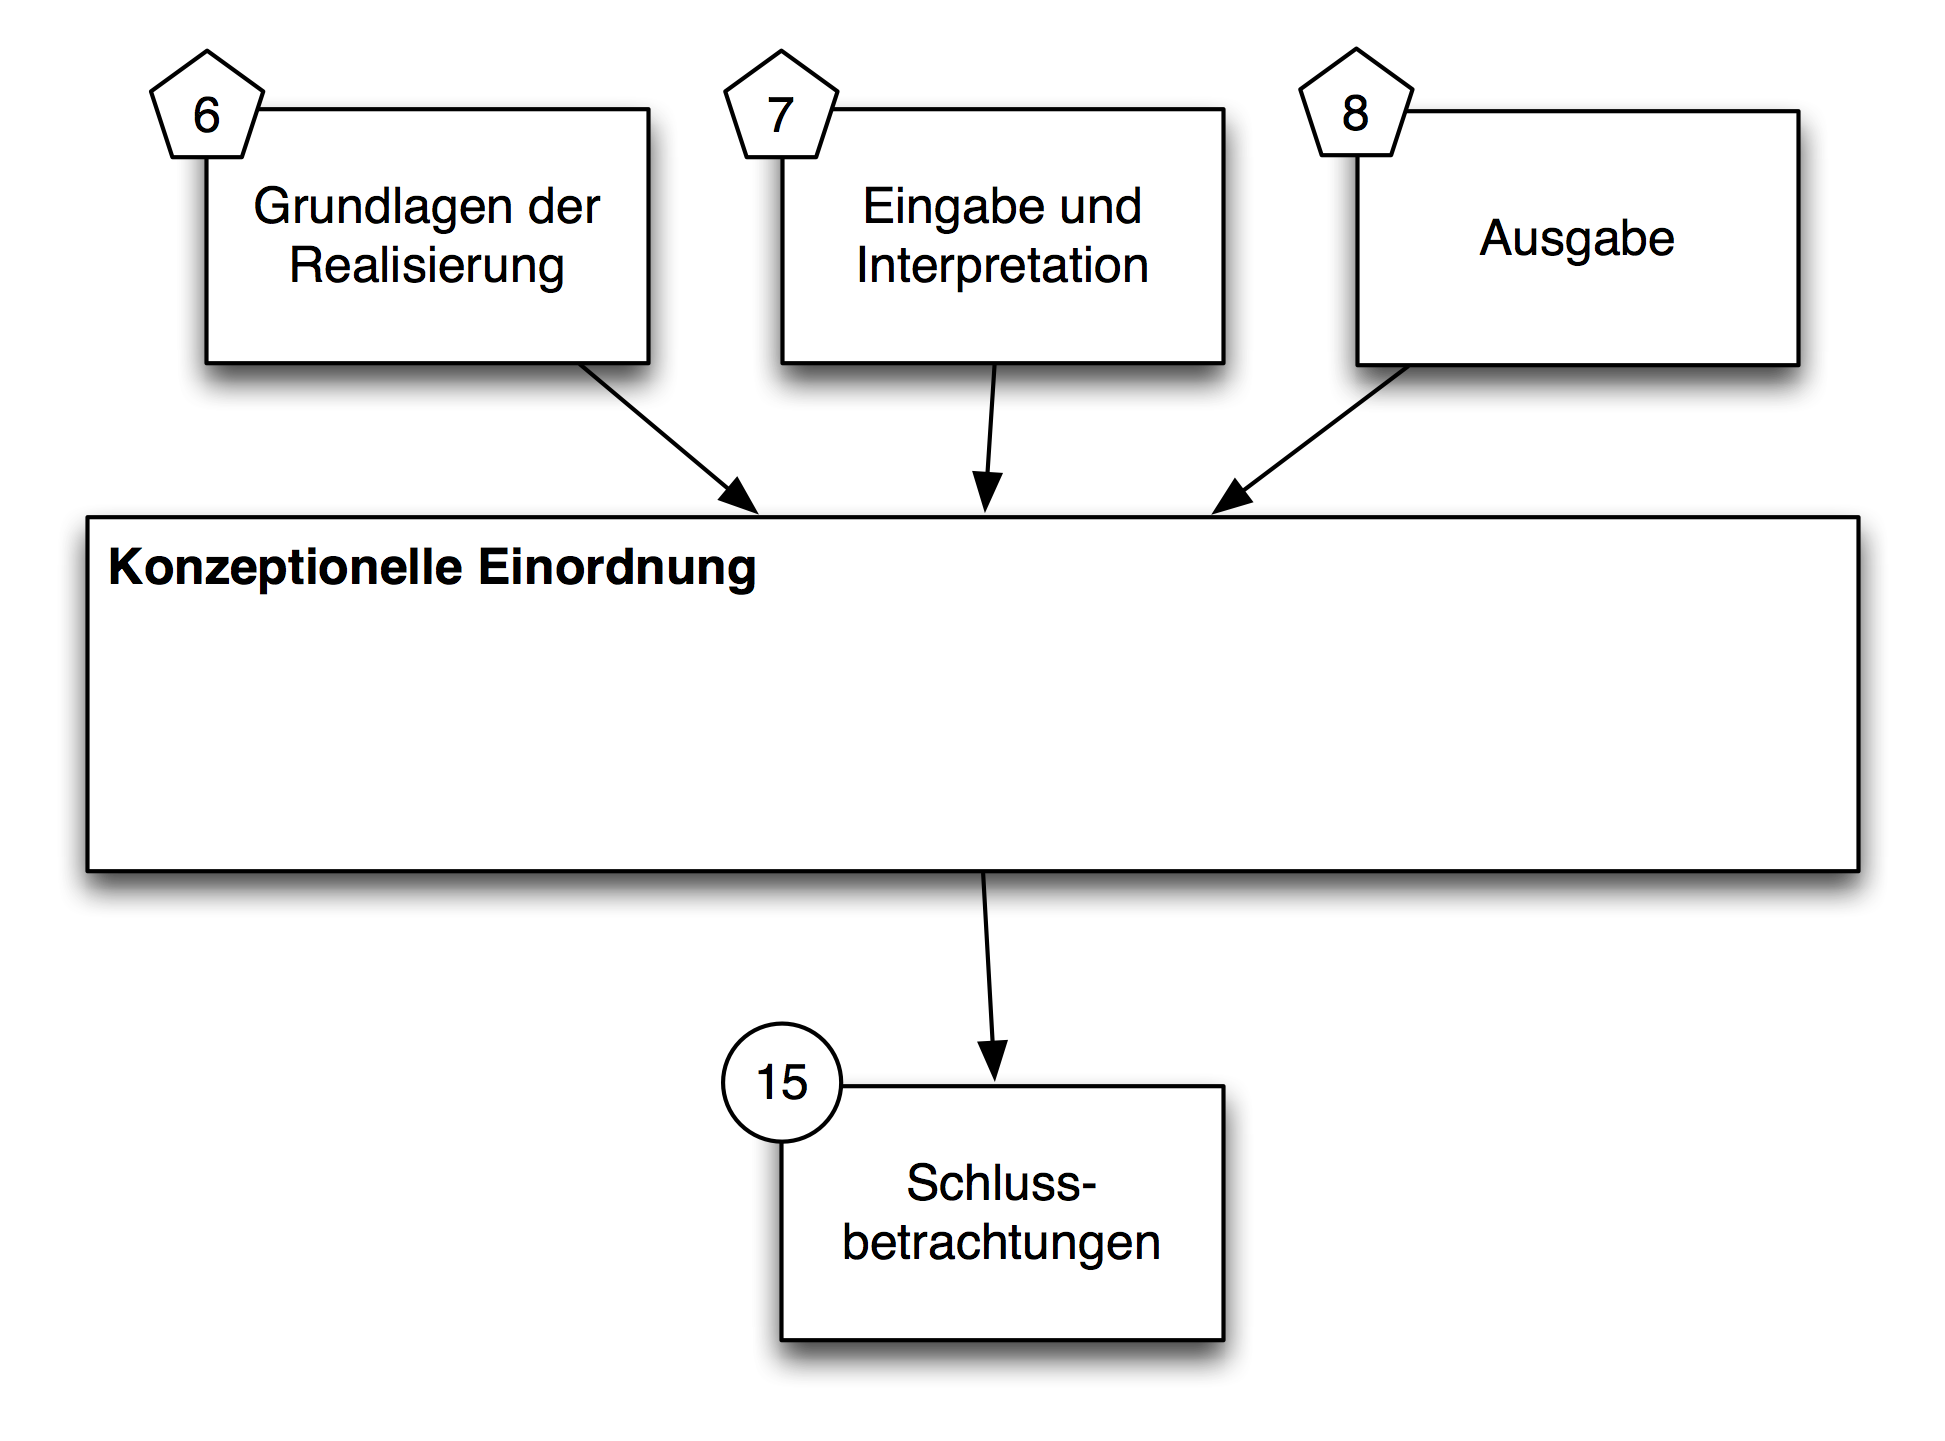
\includegraphics[scale=0.6]{img/Kontextgrafiken/k10.png}
	\caption{Kapitel „Konzeptuelle Einordnung“ im Gesamtzusammenhang}
	\label{fig:img_Kontextgrafiken_k10}
\end{figure}

Dieses Kapitel folgt im Aufbau der Struktur des Abschnitts \ref{sec:konzeptualisierungen_von_tangible_interfaces} und betrachtet in der Folge jeden der vorgestellten Ansätze in einem separaten Abschnitt. Dabei werden jeweils die Konzepte des Ansatzes auf das Werkzeug angewandt (Unterabschnitt „Abbildung“) und in der Folge die Erkenntnisse über die Eignung des Ansatzes und mögliches Verbesserungpotential des Werkzeugs angeführt (Unterabschnitt „Bewertung“). Abschließend erfolgt eine zusammenfassende Betrachtung der Ergebnisse hinsichtlich der beiden oben formulierten Ziele.

\section{Einordnung in den Bricks-Designraum} % (fold)
\label{sec:einordnung_in_den_bricks_designraum}

Grundlage der Betrachtungen in diesem Abschnitt ist das Konzept der Tangible Bits \citep{Fitzmaurice95}, der in Abschnitt \ref{sub:bricks} beschrieben wird.

\subsubsection{Abbildung} 

Aus den Erfahrungen mit der Erstellung des „Bricks“-Systems leiten \citet{Fitzmaurice95} einen  „Design Space“ ab, der 13 Merkmale definiert, die bei der Konzeption eines \gls{TUI} beachtet werden sollten bzw. die sich zum strukturierten Vergleich von \glspl{TUI} eignen. Neben den Merkmalen geben die Autoren auch mögliche Ausprägungen an, die gemeinsam den Design Raum abstecken. Für das hier vorgestellte Werkzeug ergibt sich folgende Zuordnung:

In der Kategorie \emph{Brick's internal ability} ist das System bzw. die eingesetzten Tokens als „inert“ zu klassifizieren, da die physischen Objekte keine Elektronik aufweisen und somit kein aktives Verhalten zeigen können. Bezieht man die unmittelbare Umgebung der Elemente, auf die Information projiziert werden kann, in die Beurteilung mit ein, so ist die Einstufung „simple expressions“ zu rechtfertigen. 

In der Kategorie \emph{Input \& Output} werden eingabeseitig in unterschiedlichen Interaktionen folgende Parameter kontinuierlich oder ereignisgesteuert erfasst: X-Y-Position (kont.) , Rotation (kont.) , Tastatureingabe (ereignisgest.) und Kamerabild (ereignisgest.). Ausgabeseitig werden folgende Parameter eingesetzt: Zustand auf der physischen Oberfläche, Projektion und Bildschirm.

In der Kategorie \emph{Spatially aware} ist (bezogen auf die Tokens) die Ausprägung „unaware“ zu wählen, da die physischen Elemente selbst keine Möglichkeit zur Feststellung der Konfiguration ihrer Umgebung haben. Bezogen auf das Gesamtsystem ist die Ausprägung „mutual awareness“ zu wählen, da den softwareseitigen Repräsentationen der Elemente durch das im Hintergrund arbeitende Lokalisierungssystem durchaus bekannt ist, wo sie sich befinden und welche Elemente sich in ihrer Nähe befinden.

In der Kategorie \emph{Communication} ist keine Einordnung möglich, da die physischen Elemente des Systems nicht untereinander kommunizieren.

In der Kategorie \emph{Interaction time span} sind die Ausprägungen „quick“ und „interaction cache“ zu wählen. Die meisten Interaktionen laufen ereignisbasiert ab und sind mit der Auslösung wieder abgeschlossen („quick“). Manche Interaktionen (z.B. Herstellung einer Verbindung, Kontrolle der Modellierungshistorie, \ldots) benötigen jedoch längere Zeit bzw. die Manipulation mehrerer Tokens („interaction cache“).

In der Kategorie \emph{Bricks in use at same time} ist bei Betrachtung des gesamten Systems die Ausprägung (Größenordnung) „5-10“ zu wählen, da potentiell so viele Modellierungselemente gleichzeitig (auch durch mehrere Personen) benutzt werden. Bezogen auf die Werkzeug-Tokens (also die unmittelbar funktionsauslösenden physischen Elemente, die eigentlich von diesem Ansatz eigentlich betrachtet werden) sind die Ausprägungen „1“ oder „2“ (je nach Interaktion) zu wählen.  

In der Kategorie \emph{Function assignment} ist bezogen auf die Werkzeug-Tokens die Ausprägung „permanent“ zu wählen, da diesen die durch sie ausgelöste Funktion fix zugeordnet ist.

In der Kategorie \emph{Interaction representations} ist die Ausprägung „balanced“ insofern für das vorliegende Werkzeug passend, als dass die physischen und digitalen Elemente einander in der Repräsentation des Systemzustandes gleichberechtigt ergänzen.

In der Kategorie \emph{Physical \& virtual layers} erfüllt das System durch die beiden Ausgabekanäle beide Ausprägungen („direct“ für die Tischoberfläche, „indirect“ für den sekundären Ausgabekanal).

In der Kategorie \emph{Bond between physical \& virtual layers} sind physische und virtuelle Ebene im hier vorgestellten System „tightly coupled“, da die Repräsentationen auf beiden Ebenen stets synchron sind.

In der Kategorie \emph{Operating granularity} ist aufgrund der physischen Natur des Systems (Tisch) die Ausprägung „Desktop“ zu wählen, wobei dies auch mit der vorgesehenen Auflösung des Tracking („fraction of inches accuracy“) korreliert.

In der Kategorie \emph{Operating surface type} erfüllt das System die Anforderungen der Ausprägung „dynamic“, da sich die Oberfläche durch die Projektion von Information zur Laufzeit ändert.

In der Kategorie \emph{Operating surface texture} ist die Ausprägung „continuous“ auszuwählen, da die Elemente frei auf der Oberfläche platziert werden können.

\subsubsection{Bewertung}

Der von \citet{Fitzmaurice95} aufgespannte Design Raum für Graspable User Interfaces ist aus dem von den Autoren entwickelten System abgeleitet und weist mangels zum Zeitpunkt der Erstellung vorhandenen Alternativen starke Spezifika auf, die den Ansatz zur Einordnung anderer Systeme nur bedingt geeignet machen. Insbesondere die Ableitung mehrerer Eigenschaften aus der Tatsache, dass die physischen Elemente des System (die „Bricks“) aktive Bausteine sind und auf eine Oberfläche bewegt werden, schränkt die Verwendbarkeit einiger Kategorien für die Einordnung beliebiger \glspl{TUI} ein (z.B. \emph{Communication} oder \emph{Spatially aware}). Außerdem ist der Design Raum auf Systeme ausrichtet, die physische Elemente als Eingabewerkzeuge verwenden und berücksichtigt keine Elemente, die ausschließlich zur Informationsrepräsentation verwendet werden.

Das hier vorgestellte Werkzeug konnte weitgehend in den Design Raum eingeordnet werden, wenn auch die Verwendung passiver Tokens nicht vorgesehen ist und damit einige Kategorien nicht sinnvoll belegt werden können. Ansätze zur Verbesserung des Werkzeugs können nicht abgeleitet werden, das der Designraum für Detailbetrachtungen zu unspezifisch bleibt und seine generelle Ausrichtung nicht vollständig auf die Eigenschaften des Werkzeugs abgebildet werden können.

% section einordnung_in_den_bricks_designraum (end)

\section{Bestimmung der Eigenschaften des Graspable User Interfaces Ansatz} % (fold)
\label{sec:bestimmung_der_eigenschaften_des_graspable_user_interfaces_ansatz}

Grundlage der Betrachtungen in diesem Abschnitt ist das Konzept der Tangible Bits \citep{Fitzmaurice96}, der in Abschnitt \ref{sub:graspable_user_interfaces} beschrieben wird.

\subsubsection{Abbildung}

\citet{Fitzmaurice96} definiert fünf Eigenschaften, die ein „Graspable User Interface“ ausmachen und legt mögliche Ausprägungen fest, deren Werte für ein konkretes System eine Aussage über dessen „Graspabiltity“ zulässt. Für das hier vorgestellte Werkzeug sind folgende Einstufungen argumentierbar:

In der Kategorie \emph{Space-multiplexing} ist die höchste Ausprägung „permanent, never reassign“ auszuwählen. Dies ist der Fall, weil sämtlichen Werkzeugtokens des Systems eine vorgegebene Funktion zugewiesen ist, die sich während der Laufzeit nicht ändert.

In der Kategorie \emph{Concurrency} ist hinsichtlich der Verwendung von Werkzeugen die Ausprägung „occasionally 2“ zu wählen. Die Eigenschaften beziehen sich ausschließlich auf Werkzeuge zur Manipulation digitaler Information, so dass die Modellierungstokens, die den Systemzustand repräsentieren, außer acht gelassen werden. „Occasionally 2“ trifft dann deswegen zu, weil sowohl bei der Verbindungsherstellung als auch zum Auslösen der Wiederherstellungsunterstützung jeweils zwei Werkzeugtokens gleichzeitig eingesetzt werden müssen, in allen anderen Fällen aber nur ein Werkzeug zum Einsatz kommt. Berücksichtigt man die Modellierungstokens (als Werkzeuge zur Manipulation des Systemzustandes), wäre die höchste Ausprägung „more than 3“ zu wählen.

In der Kategorie \emph{Physical form} ist die höhere Ausprägung „specific“ auszuwählen, da für jede Funktionalität ein spezifisches Werkzeug-Token existiert.

In der Kategorie \emph{Spatially aware} ist hinsichtlich der Werkzeugtokens eine Mischform zwischen „unaware“ und „aware“ zu wählen. Bei einem Teil der Werkzeugtokens ist die konkret ausgeführte Funktion von dessen Position bzw. Nähe zu Modellierungstokens abhängig (bei Markierungstokens) oder wird durch dessen Orientierung beeinflusst (beim Historien-Kontroll-Token). Die übrigen Werkzeug-Tokens sind jedoch insofern „spatially unaware“, als das ihre Positionierung auf der Oberfläche keinen Einfluss auf deren Funktionalität hat. Die Modellierungstokens und die einbettbaren Tokens wären bei Berücksichtigung als „spatially aware“ zu klassifizieren.

In der Kategorie \emph{Spatial reconfiguarability} ist das System in die Ausprägung „track“ einzuordnen, da die einzelnen Werkzeuge nicht unabhängig von der Oberfläche und der in ihr integrierten optischen Tracking-Funktion verwendet werden können.

\subsubsection{Bewertung}

Die Eigenschaften von Graspable User Interfaces erlauben eine allgemeine Bewertung eines \gls{TUI}. Sie sind nicht geeignet, um eine detailliert Analyse oder Spezifikation durchzuführen. Dieser Aspekt -- die Eigenschaften des Gesamtsystems -- wird jedoch bei den meisten anderen Frameworks außer acht gelassen, so dass eine Einordung in das vorgeschlagene Schema durchaus sinnvoll sein kann.

Für das hier vorgestellte Werkzeug wurden durchwegs Ausprägungen identifiziert, die auf eher hohe „Graspability“ hinweisen. Ein Nachteil des Ansatzes liegt in der Fokussierung auf reine „Steuerungs“-\glspl{TUI}, die zur Kontrolle oder Manipulation digitaler Information verwendet werden. Würde der Repräsentations-Aspekt eines \gls{TUI} (stärker) berücksichtigt, würden sich, wie oben beschrieben, zum Teil höhere Ausprägungen in einzelnen Kategorien ergeben. Verbesserungspotential kann ob der allgemeinen und relativ abstrakten Beschreibung des Werkzeugs mit diesem Ansatz nicht abgeleitet werden.

% section bestimmung_der_eigenschaften_des_graspable_user_interfaces_ansatz (end)

\section{Betrachtung im Lichte des Tangible Bits Ansatzes} % (fold)
\label{sec:betrachtung_tangible_bits}

Grundlage der Betrachtungen in diesem Abschnitt ist das Konzept der Tangible Bits \citep{Ishii97}, der in Abschnitt \ref{sub:tangible_bits} beschrieben wird.

\subsubsection{Abbildung} 

Das hier vorgestellte Werkzeug kann hinsichtlich seiner Funktion als eine Instanz des Konzepts „Interactive Surface“ betrachtet werden. Die „Surface“ ist hierbei eine Tischoberfläche, auf der interagiert wird. Die im Rahmen der Beschreibung des „metaDESK“ \citep{Ullmer97} als Beispiel für eine „Interactive Surface“ eingeführten \gls{TUI}-Elemente finden zum Teil auch im hier vorgestellten Werkzeug Anwendung.

Die Modellierungstokens und einbettbaren Tokens des Werkzeugs sind \emph{Phicons}, also passive Träger von digitaler Information. Die Werkzeugtokens zur Manipulation des Modells entsprechen \emph{Phandles}, also Elemente, die dazu verwendet werden, digitale Information zu verändern bzw. festzulegen. Jene Werkzeugtokens, die der Steuerung der Systemfunktionen dienen, sind hingegen als \emph{Instruments} zu klassifizieren. \emph{Lenses} und \emph{Trays} kommen im Werkzeug nicht zum Einsatz.

Hinsichtlich der Metaphorik unterscheiden \citet{Ullmer97} zwischen unterschiedlichen Abstraktionsebenen von Phicons (\emph{generic} -- \emph{symbolic} -- \emph{model}), wobei im vorliegenden System ob der offenen Semantik die Modellierungstokens ausschließlich \emph{generic Phicons} sind bzw. sein können. Die Werkzeugtokens sind zumeist als \emph{symbolic Phicons} und im Falle des Löschtokens -- dem Radiergummi -- eher als \emph{model Phyicon} zu klassifizieren.

\subsubsection{Bewertung} 

Für die Bewertung des Werkzeugs ist vor allem dessen Gegenüberstellung zu den vorgeschlagenen Elementen einer „Interactive Surface“ von Interesse. Hier zeigt sich, das die unterschiedlichen Arten von Tokens, die im Werkzeug eingeführt wurden, feingranular auf die unterschiedlichen Element-Arten von \citep{Ishii97} abbildbar sind. Insbesondere die explizite Unterscheidung zwischen \emph{Phandles} und \emph{Instruments} ist ein Alleinstellungsmerkmal der hier vorgeschlagenen Systematik.

Eine mögliche Lücke, die Erweiterungspotential für das Werkzeug anzeigen könnte, ist die Abwesenheit von TUI-Elementen, die als \emph{Lenses} oder \emph{Trays} zu klassifizieren sind. Insbesondere \emph{Trays} erscheinen für die explizite Interaktion mit einzelnen Tokens -- etwa der Benennung oder der Einbettung von Zusatzinformation -- als geeignet. Die dazu notwendigen Interaktionsabläufe würden expliziter auf den Vorgang der Zuordnung von Information eingehen und sich stärken von anderen Interaktionen unterscheiden, die anderen Zwecken, z.B. der Herstellung von Verbindungen zwischen Modellierungstokens, dienen.

% section betrachtung_tangible_bits (end)

\section{Einordnung in das Ordnungssystem von Holmquist et al.} % (fold)
\label{sec:einordnung_in_das_ordnungssystem_von_holmquist_et_al_}

Grundlage der Einordnung in diesem Abschnitt ist der Ansatz von \citep{Holmquist99}, der in Abschnitt \ref{sub:containers_tokens_tools} beschrieben wurde.

\subsubsection{Abbildung}

Die von \citeauthor{Holmquist99} verwendete Terminologie ist direkt auf jene abbildbar, die in dieser Arbeit verwendet wurde. Die Modellierungstokens und einbettbaren Tokens entsprechen im Wesentlichen \emph{Tokens}. Dies ist dadurch begründbar, dass die Art eines Modellierungstokens in einem Modell immer im gleichen Zusammenhang mit der Art der Information steht, die durch dieses repräsentiert wird. Eine Eigenschaft, die eher \emph{Containern} zuzuordnen ist, ist jedoch die dynamische Festlegbarkeit der Bedeutung einer Art von Modellierungstokens - die physischen Elemente an sich sind vor Beginn der Modellbildung generisch (also \emph{Container}), werden aber im Zuge der Modellierung mit Bedeutung belegt (die dann für alle Instanzen dieser Art von Modellierungstokens gilt) und sind dann eher als \emph{Tokens} zu klassifizieren. 

Die Werkzeugtokens des hier vorgestellten Systems entsprechen in ihrer Konzeption den \emph{Tools}. Sie manipulieren digitale Information, lösen Aktionen aus oder versetzten das System in einen anderen Zustand und entsprechen damit exakt der Definition von \emph{Tools}, die von den Autoren gegeben wird.

\emph{Information Faucets} sind im Kontext des hier vorgestellten Systems einerseits die Tischoberfläche, über die Information zu Modellierungstokens abgerufen werden kann, andererseits ist die Registrierungskamera ein klassisches Faucet im Sinne der Definition, da sie dem Abruf oder der Assoziation von Information an ein Token dient, sobald dieses in den Erfassungsbereich der Kamera gerät.

\subsubsection{Bewertung}

Die konzeptuellen Elemente des hier vorgestellten Systems sind also auf das Ordnungssystem von \citet{Holmquist99} abbildbar. Die Problematik der nicht eindeutigen Zuordnung von Modellierungstokens zur Kategorie \emph{Tokens} oder \emph{Constraints} ist einerseits auf eine der grundlegenden Design-Paradigmen des hier entwickelten Werkzeugs -- der Flexibilität der Abbildung -- zurückzuführen, weist aber andererseits auch auf mögliches Verbesserungspotential hin.

Durch die Flexibilisierung nicht nur der Bindung zwischen physischen Elementen und digitaler Repräsentation sondern auch der Verwendung von unterschiedlichen physischen Elementen selbst könnten Modellierungstokens eher \emph{Token}-artiger werden. Indem Modellierende eigene physische Elemente (auf ihrem Arbeitskontext) einbringen können, könnte die Erfassbarkeit der Bedeutung der physischen Repräsentation unter Umständen verbessert werden können.

% section einordnung_in_das_ordnungssystem_von_holmquist_et_al_ (end)

\section{Einordnung in das Object-Meaning-Kontinuum} % (fold)
\label{sec:einordnung_in_das_object_meaning_kontinuum}

Grundlage der Einordnung in diesem Abschnitt ist der Ansatz von \citet{Underkoffler99}, der in Abschnitt \ref{sub:tangible_objects_meaning} beschrieben wurde.

\subsubsection{Abbildung} 

Das Object-Meaning-Kontinuum ist einer der ersten Ansätze, die die physischen Objekte eines \gls{TUI} nicht strikten Kategorien zuordnen sondern auf einer kontinuierlichen Skala anordnen. Dabei wird kein kategorischer Unterschied zwischen informationsrepräsentierenden Objekten und Werkzeug-Objekten gemacht -- sowohl in der Mitte des Kontinuums als auch an den Enden verschwimmen die Grenzen zwischen dem Verständnis eines Objektes als reine Repräsentation und reinem Werkzeug. 

In der Folge werden die Elemente des Werkzeugs in das Kontinuum eingeordnet, wobei zur einfacheren Anwendbarkeit die entlang des Kontinuums von den Autoren definierten Ausprägungen verwendet werden.

Die Ausprägung \emph{object as noun} kommt im Werkzeug nicht zum Einsatz. Keines der physischen Elemente hat eine direkte Entsprechung in der realen Welt -- durch die geforderte Flexibilität der Abbildung wäre das auch nicht sinnvoll. 

Die Elemente die zur Modellbildung verwendet werden -- also Modellierungstokens und einbettbare Tokens -- sind der Ausprägung \emph{object as attribute} zuzuordnen, da in die Farbe bzw. Form der Tokens Bedeutung (nämlich die Semantik des jeweiligen Art von Tokens) codiert ist. Bei Modellierungstokens ist zu beachten, dass die Zuordnung der Bedeutung dynamisch zu Laufzeit erfolgt, der physischen Eigenschaft des Objekts also erst durch die Benutzer konkret Bedeutung zugewiesen wird.

Keines der Objekte des Werkzeug ist aufgrund seines Designs der Ausprägung \emph{object as pure object} zuzuweisen. Diese Zuordnung kann jedoch dynamisch bei der Modellbildung für Modellierungstokens eintreten, wenn die Benutzer den unterschiedlichen Objektarten keine Bedeutung zuordnen und diese beliebig mit Information belegen. 

Die Tokens, die im Werkzeug nicht unmittelbar zur Modellbildung verwendet werden, verteilen sich zwischen den beiden funktional abstrahierten Ausprägungen des Kontinuums. Der Ausprägung \emph{Object as Verb} sind das Historiensteuerungs-Token und das Markierungstoken zur Herstellung einer gerichteten Verbindung zuzuordnen. Für das Historiensteuerungs-Token gilt dies, da dessen Drehbewegung zur zeitliche Navigation auf die Bewegungen eines Uhrzeigers abbildbar ist. Das Markierungstoken zur Herstellung einer gerichteten Verbindung weist eine Pfeilspitze als Grundfläche auf, wodurch eine physische Eigenschaft Hinweise auf die Funktion des Tokens gibt (hier allerdings grenzwertig, das die dreieckige Grundfläche nicht eindeutig als Pfeilspitze zu erkennen ist). Die übrigen Tokens sind eher im Bereich des \emph{object as reconfigurable tool} anzusiedeln, da ihrer äußere Form oder ander physische Eigenschaften keine Hinweise auf deren Funktionalität geben. Dies gilt für die allgemeinen Markierungstokens, das Snaphshot-Token und das Wieder\-herstellungs-Token. 

Einen Spezialfall bildet das Löschtoken, das mit dem Radiergummi als Repräsentation eine \emph{object as verb}-Einordnung suggeriert (Radiergummi zum direkten „Ausradieren“ von Verbindungen), tatsächlich das System aber lediglich in einen Löschmodus versetzt, in dem Verbindungen mittels anderer Interaktionsabläufe gelöscht werden können. Hinsichtlich seiner tatsächlichen Verwendung ist das Löschtoken also als \emph{object as reconfigurable tool} zu klassifizieren.

\subsubsection{Bewertung} 

Das von den Autoren vorgeschlagene Kontinuum eignet sich, um die Elemente eines \gls{TUI} hinsichtlich deren Bedeutung und Verwendung einzuordnen. Diese Einordnung kann nützlich sein, um Elemente zu identifizieren, deren tatsächliche Verwendung im TUI nicht mit der wahrgenommenen Bedeutung übereinstimmt. Dazu müssen die Elemente unabhängig von der konkreten Implementierung klassifiziert werden (ggf. von nicht am Design und der Entwicklung beteiligten Personen) und das Ergebnis der umgesetzten Funktionalität gegenübergestellt werden.

Für das hier vorgestellte Werkzeug ist eine derartige Diskrepanz wie oben bereits beschrieben am Löschtoken zu erkennen. Dieses suggeriert eine Verwendbarkeit im Sinne von \emph{object as verb}, setzt aber tatsächlich die augenscheinliche Funktion (Löschen) nicht um (bzw. ist auf eine andere Funktion -- Löschmodus aktivieren -- abgebildet) und ist deshalb lediglich als \emph{object as reconfigurable tool} einzuordnen. Eine „Aufwertung“ des Löschtokens im Sinne einer Hinterlegung mit der tatsächlichen Lösch-Funkton würde eine erwartungskonforme Verwendbarkeit eher sicherstellen und so zur Verbesserung des Gesamtsystems beitragen.

% section einordnung_in_das_object_meaning_kontinuum (end)

\section{Betrachtung im Lichte des MCRpd-Modells} % (fold)
\label{sec:betrachtung_im_lichte_des_mcrpd_modells}

Grundlage der Einordnung in diesem Abschnitt ist der Ansatz von \citet{Ullmer00}, der in Abschnitt \ref{sub:mcrpd} beschrieben wurde.

\subsubsection{Abbildung}

Wird das erstellte Werkzeug dem \gls{MCRpd}-Modell gegenübergestellt, so ist erkennbar, das die Eigenschaften des Werkzeugs augenscheinlich nicht den Anforderungen des \gls{MCRpd}-Modells an ein Tangible User Interface genügen. Das Werkzeug verfügt über einen Ausgabekanal -- den Bildschirm -- der nicht an die physische Repräsentation gekoppelte ist. Bei näherer Betrachtung erscheint eine vollständige Einordnung jedoch argumentierbar. All jene Interaktionen, die mit der eigentlichen Modellierung zusammenhängen, genügen den Anforderungen des \gls{MCRpd}-Modells ohne Einschränkungen. Die Manipulation des \emph{Model} (im \gls{MCRpd}-Modell) erfolgt über die Tischoberfläche, die gleichzeitig dazu verwendet wird, den Systemzustand zu manifestieren. Dem \gls{MCRpd}-Modell entgegenzulaufen scheinen jene Interaktionsabläufe, die den sekundären Ausgabekanal einbeziehen. Dabei sind zwei Fälle zu unterscheiden. Bei der Einbettung von Information in Modellelemente wird die sekundäre Oberfläche zur Auswahl der anzubindenden Ressource und damit als \gls{GUI} benutzt. Eine Einordnung in das \gls{MCRpd}-Modell ist hier damit nicht möglich. Bei der Betrachtung der Modellierungshistorie wird die sekundäre Oberfläche als alleiniges Ausgabemedium benutzt, der Systemzustand wird durch das runde Navigationstoken auf der Oberfläche beeinflusst. Dies verletzt grundsätzlich den Aufbau des MCRpd-Modells.

Betrachtet man jedoch die daraus abgeleiteten Kern-Charakteristika von \glspl{TUI}, so kann festgestellt werden, das diese dennoch nicht verletzt sind. Das in Frage zu stellende Charakteristikum ist jene mit der Forderung nach Kopplung zwischen der physischen Repräsentation des \emph{Models} (\emph{REP-P}) und der intangiblen, digitalen Manifestation von Modellaspekten in der realen Welt (\emph{REP-D}). Die Autoren fordern von dem Zusammenhand zwischen \emph{REP-P} und \emph{REP-D} jedoch ausschließlich, dass er \emph{„perceptually coupled“} sein müsse, die Kopplung also von den Benutzern als solche wahrgenommen werden müsse. Betrachtet man das runde Navigationstoken als \emph{REP-P} und die Ausgabe am sekundären Ausgabekanal als \emph{REP-D}, so ist diese Kopplung feststellbar, da sich \emph{REP-D} immer in direkter Abhängigkeit von \emph{REP-P} verändert. Insofern ist das \gls{MCRpd}-Modell nicht verletzt, das Werkzeug weist die von den Autoren als Kern-Charakteristika von Tangible User Interfaces bezeichneten Eigenschaften auf.

Hinsichtlich der Kategorien von \glspl{TUI}, die von den Autoren festgelegt werden, ist das System der Kategorie \emph{relational} zuzuordnen. Das hier vorgestellte Werkzeug ist nicht \emph{spatial}, da die Position der verwendeten Tokens relativ zum Referenzrahmen (der Tischoberfläche) keine spezifische Bedeutung haben. Die Bedeutung ist viel mehr in den Beziehungen der Tokens untereinander codiert, was wiederum für ein \emph{relationales} System sprechen würde. Gleichzeitig kann damit die Kategorie \emph{associative} ausgeschlossen werden, da in Systemen dieser Art keine Beziehungen zwischen Tokens berücksichtigt werden. Da die Beziehungen zwischen Tokens nur digital und nicht physisch abgebildet werden, ist die Bedingung für ein \emph{konstruierendes} System nicht erfüllt. \emph{Constructive} wäre das Werkzeug dann, wenn der Modellzustand vollständig durch physische Elemente und Verbindungen abgebildet wäre.

\subsubsection{Bewertung}

Das \emph{MCRpd}-Modell ist ein im Vergleich zu anderen Ansätzen eher abstraktes, konzeptuelles Modell zur Beschreibung eines Tangible User Interfaces. Trotzdem -- oder auch deswegen -- eignet es sich gut zur Reflexion der Eigenschaften eines \glspl{TUI} bzw. zur Prüfung der Konsistenz der vorgesehenen Benutzerinteraktionen.

Das Werkzeug konnte in die Logik des Modells eingeordnet werden, wobei bei der Beschreibung der Interaktion zur Steuerung der Modellierungshistorie verstärkter Argumentationsbedarf herrschte. Dies kann auf eine möglicherweise zu schwache Kopplung zwischen \emph{REP-P} und \emph{REP-D} hinweisen. Tatsächlich wird bei der Kontrolle der Modellierungshistorie auf der Tischoberfläche kein Feedback ausgegeben, ob das Steuerungs-Token erkannt wurde und in welchem Zustand es sich aktuell befindet. Die Kopplung könnte etwa in Form einer Darstellung des aktuell dargestellten Zeitpunkts in der Modellierungshistorie rund um das Kontroll-Token angezeigt werden, was die Kopplung zwischen den beiden Komponenten der Repräsentation verstärken würde.

% section betrachtung_im_lichte_des_mcrpd_modells (end)

\section{Einordnung in den Tokens+Constraints Kontext} % (fold)
\label{sec:einordnung_in_den_tokens_constraints_kontext}

Grundlage der Einordnung in diesem Abschnitt ist der Ansatzes von \citep{Ullmer05}, der in Abschnitt \ref{sub:tokens_und_constraints_nach_ullmer} beschrieben wurde.

\subsubsection{Einordnung}

Eine unmittelbare Einordnung des hier vorgestellten Werkzeugs in den Tokens+Constraints-Ansatz ist nicht möglich, da einerseits kein allgemeines Schema zur Betrachtung vorgeschlagen wird und das Werkzeug seiner Konzeption nach nicht dem Verständnis eines Tokens+Constraints-System nach \citep{Ullmer05} entspricht. Dazu müsste es physische Constraints aufweisen, die den Interaktionsraum der informationstragenden Tokens physisch einschränken. Das einzige nach dieser Definition identifizierbare Constraint des Werkzeugs ist der aktive Bereich der Tischoberfläche, die den Modellierungsraum beschränkt. Diese Einschränkung ist aber im Vergleich zu den Beispielen für Constraints, die die Autoren angeben, eher wenig strikt und lässt viel Interaktionsraum.

Am ehesten ist das vorliegende System als eine „interactive surface“ mit Aspekten einer „constructive assembly“ zu klassifizieren. Die Qualifikation als „interactive surface“ erscheint ob der Interaktion mit physischen Blöcken auf einer digital augmentierten Oberfläche naheliegend. „Constructive assembly“-Aspekte sind im Bereich der Einbettung von informationstragenden Tokens in Modellierungs-Tokens zu finden. Die Zuordnung wird dabei durch das Hineinlegen eines Tokens in ein anderes ausgedrückt, wodurch die konkrete Semantik in der Beziehung zwischen den beiden Tokens abgebildet ist. Generell wird die Semantik des abzubildenden Modells in der räumlichen und logischen Konfiguration der Modellierungs-Tokens zueinander abgebildet, was ebenfalls einem „constructive assembly“-Aspekt entspricht.

Nicht unmittelbar in in Zusammenhang mit dem Tokens+Constraints-Ansatz stehen die fünf Fragen von \citep{Bellotti02}, die beim Design einer Benutzungsschnittstelle berücksichtigt werden sollten. In \citet{Ullmer05} werden diese Fragen für den dort vorgestellten Ansatz beantwortet, an dieser Stelle sollen sie im Lichte des hier vorgestellten Systems betrachtet werden.

\begin{description}
	\item[Address] Das System interpretiert alle Interaktionen, die mit Modellierungs- oder Werkzeugtokens unmittelbar auf der Tischoberfläche ausgeführt werden, als an es gerichtet. Andere Interaktionen werden ignoriert und können auch technisch nicht erfasst werden.
	\item[Attention] Der Einsatz jedes Tokens löst unmittelbar eine Reaktion auf den Ausgabekanälen des Systems aus. Benutzer erhalten also direktes Feedback auf erkannte Interaktionen. Eine Verzögerung zwischen Ein- und Ausgabe tritt lediglich bei der Markierung von Elementen auf, die zur Robustheit gegen Fehlerkennungen erst erfasst wird, wenn das  Eingabe-Token länger als 500 ms vorhanden ist.
	\item[Action] Befehle an das System können generell an einem beliebigen Punkt der Oberfläche abgesetzt werden, sofern es sich um allgemeine Kommandos handelt, die das Gesamtsystem betreffen. Befehle, die einem bestimmten Objekt zuzuordnen sind (z.B. Auswahl oder Verbindungsherstellung) werden durch räumliche Nähe zugeordnet.
	\item[Alignment] Nach Ausführung einer Aktion befindet sich das System immer in einem stabilen Zustand, anhand dessen Visualisierung die Benutzer erkennen können, ob die intendierte Aktion korrekt erkannt und ausgeführt wurde.
	\item[Accident] Missverständnisse zwischen System und Benutzern können auf unterschiedliche Arten aufgelöst werden. Die erste Möglichkeit ist, Missverständnisse explizit durch die gegenteilige Interaktion rückgängig gemacht werden (z.B. Löschen einer versehentlich hergestellten Verbindung). Mittels der Wiederherstellung eines gespeicherten Systemzustandes kann ein Missverständnis ebenfalls korrigiert werden.
\end{description}

\subsubsection{Bewertung}

Der Tokens+Constraints-Ansatz ermöglicht in der vorliegenden Form keine direkte Abbildung des Werkzeugs auf seine Konzepte. Wertvoller für die Betrachtung sind an dieser Stelle die Ordnungsschemata und Fragestellungen, die von \citet{Ullmer05} im Kontext des Ansatzes erarbeitet bzw. beantwortet werden. 

Von Interesse sind insbesondere die fünf Fragen für das Design von Benutzungsschnittstellen, die von  \citep{Bellotti02} gestellt werden. Bei der Beantwortung dieser Fragen für das vorliegende System ist durchaus Verbesserungspotential zu identifizieren. Am offensichtlichsten zeigt sich das am Beispiel des Feedbacks des Systems an Benutzer über einen erkannten Interaktionswunsch. Hier kommt es beim Einsatz des Markierungstokens technisch bedingt zu Verzögerungen, die -- ob der ansonsten unmittelbaren Reaktion des Systems -- Unsicherheit bei den Benutzern erzeugen kann. Auch die Auflösung von Missverständnissen ist im Moment sub-optimal gelöst, da in jedem Fall entweder Zeitverlust auftritt oder mindestens zwei Interaktionsschritte zur Korrektur einer Fehlinterpretation notwendig sind. Hier wäre unter Umständen die Einführung einer expliziten „Undo“-Funktionalität sinnvoll.

% section einordnung_in_den_tokens_constraints_kontext (end)

\section{Einordnung in das Framework nach Koleva et al.} % (fold)
\label{sec:einordnung_in_das_framework_nach_koleva_et_al_}

Grundlage der Einordnung in diesem Abschnitt ist der Ansatzes von \citep{Koleva03}, der in Abschnitt \ref{sub:degree_of_coherence} beschrieben wurde.

\subsubsection{Abbildung} % (fold)
\label{sub:abbildung}

Das Framework eignet sich zur Einordnung einzelner Aspekte eines Tangible User Interfaces. Aufgrund seiner Ausrichtung auf die Brücke zwischen realer und digitaler Welt ist es insbesondere für die Betrachtung der eingesetzten Tokens und deren Verwendung zur Repräsentation und Manipulation des Systemzustandes geeignet. In Tabelle \ref{tab:degree_of_coherence} werden die Tokens in die Kategorien entlang des Kohärenz-Kontinuums eingeordnet und hinsichtlich der Eigenschaften ihrer Brückenfunktion in die digitale Welt betrachtet. 

\begin{table}[htbp]
	\centering
	\caption{Beurteilung des Werkzeugs hinsichtlich des Degree of Coherence}
	\begin{tabular}{| p{2cm} || p{2cm} | p{1,2cm} | p{2,5cm} | p{1,5cm} | p{1,2cm} | p{1,2cm} |} \hline
		Element & Kategorie & Trans\-for\-mation & Sensing of Inter\-action & Konfig\-urierbar\-keit & Lebens\-dauer & Auto\-nomie \\ \hline \hline
		Modell\-ierungs\-token  & Proxy & lit. & X-Y-Position und Rotation, Öffnungsstatus & fixiert & temp. & abh. \\ \hline
		einbett\-bares Token & Identifier & transf. & Präsenz, Container & fixiert & temp. & unabh. \\ \hline
		Mark\-ierungs\-token & Specialized Tool & transf. & X-Y-Position & fixiert & temp. & unabh. \\ \hline
		Löschtoken & Projection & transf. & Präsenz & fixiert & perm. & unabh. \\ \hline
		Snapshot\-token & Specialized Tool & transf. & Präsenz & fixiert & perm. & unabh. \\ \hline
		Historien\-navigations\-token & Specialized Tool & transf. & Rotation & fixiert & perm. & unabh. \\ \hline
		Wieder\-herstellungs\-token & Specialized Tool & transf. & Präsenz & fixiert & perm. & unabh. \\ \hline
	\end{tabular} \\
	\footnotesize lit. \ldots literally, transf. \ldots transformed, konfig. \ldots konfigurierbar, temp. \ldots temporär,\\ perm. \ldots permanent, abh. \ldots abhängig, unabh. \ldots unabhängig
	\label{tab:degree_of_coherence}
\end{table}

Die Kardinalität wurde hier nicht gesondert betrachtet, die diese im vorliegenden System immer 1:1 ist, also eine eindeutige Zuordnung zwischen realem Objekt und digitaler Repräsentation gegeben ist. Im Übrigen verzichten auch \citet{Koleva03} auf die Einordnung in diese Kategorie, da sie generell nur geringe Unterscheidungskraft aufweist. Hinsichtlich der „Source of Link“, die in der Tabelle ebenfalls nicht angegeben ist (und von den Autoren ebenfalls nicht verwendet wird), ist anzumerken, dass das Werkzeug durchaus einen Aspekt aufweist, bei dem der „Source of Link“ die digitale Welt ist. Im Rahmen der Wiederherstellungsunterstützung gibt das System Anweisungen zur Manipulation der realen Welt, wodurch sich der Informationsfluss umkehrt. Da jedoch kein physisches Element direkt manipuliert wird, ist eine Einordnung in das oben angeführte Schema nicht möglich (der Link ist lediglich indirekt vorhanden).

% subsection abbildung (end)

\subsubsection{Bewertung} % (fold)
\label{sub:bewertung}

Das von \citep{Koleva03} vorgeschlagene Framework ermöglicht die Klassifikation eines Tangible Interface durch die Beurteilung der Stärke der Bindung zwischen digitaler und realer Welt. Die Autoren nehmen damit eine zum Zeitpunkt der Publikation neue Perspektive ein, der bis dato noch keine große Aufmerksamkeit geschenkt wurde. Durch die Vernachlässigung der Interaktion am Tangible User Interface bildet eine Analyse unter Einsatz der im Framework vorgeschlagenen Kategorien nur einen Teilaspekt des Gesamtsystems ab. Trotz dieser Einschränkung bietet das Framework ob seiner detaillieren Betrachtung der Eigenschaften der Verknüpfung von physischen Objekten mit digitaler Information potentiell einen Mehrwert dar beim Design oder der Analyse von \glspl{TUI}. 

Insbesondere ermöglicht das Framework, nicht ausgeschöpftes Kohärenz-Potential zu identifizieren. Im konkreten Fall des hier vorgestellten Werkzeugs lässt sich das am Beispiel des Löschtokens zeigen. Dieses physisch durch einen Radiergummi repräsentierte Token wird im Moment lediglich als Schalter verwendet. Das System wird in den Löschmodus versetzt, sobald das Token auf der Oberfläche erkannt wird. Das Token ist als \emph{Projection} einzuordnen, die das Token mit der Information des aktivierten oder deaktivierten Löschmodus verbindet. Obwohl hoch kohärent, ist das Token trotzdem suboptimal eingesetzt, da es in der Praxis als Werkzeug wahrgenommen wird, das zum Löschen einer spezifischen Verbindung verwendet werden kann (\emph{Specialized Tool}). An diesem Beispiel lassen sich zwei Aspekte zeigen, die bei der Verwendung des Frameworks beachtet werden müssen. Zum einen ist hohe Kohärenz nicht für jeden Anwendungsfall erstrebenswert, da bei Werkzeugen im Allgemeinen eine nicht permanente Bindung verwendet wird. Zum anderen zeigt sich die Unvollständigkeit der Analyse mittels dem Framework, da die Metaphorik des physischen Elements, also seine Bedeutung in der Interaktion, nicht berücksichtigt wird. Beide Aspekte -- Kohärenz und Metaphorik -- berücksichtigt erst \citet{Fishkin04} in der von ihm vorgeschlagenen Taxonomie (siehe dazu die Abschnitte \ref{sub:taxonomie_fishkin} und \ref{sec:einordnung_in_die_taxonomie_von_fishkin}).

% subsection bewertung (end)
% section einordnung_in_das_framework_nach_koleva_et_al_ (end)

\section{Spezifikation des TAC-Schemas nach Shaer et al.} % (fold)
\label{sec:spezifikation_des_tac_schemas_nach_shaer_et_al_}

Grundlage der Einordnung in diesem Abschnitt ist der Ansatzes von \citet{Shaer04}, der in Abschnitt \ref{sub:tokens_und_constraints_nach_shaer_et_al_} beschrieben wurde.

\subsubsection{Abbildung}

Das „Token and Constraints“-Schema (\gls{TAC}) erlaubt es, ein Tangible Interface sowohl hinsichtliche dessen Struktur als auch dessen Verwendung zu beschreiben. In den Tabellen \ref{tab:tac1} und \ref{tab:tac2} wird das Schema auf das hier vorgestellte Werkzeug angewandt. 

\begin{table}[htbp]
	\centering
	\caption{Spezifikation des Werkzeug mittels TAC-Schema -- Teil 1}
\begin{tabular}{| p{0.8cm} || p{2.2cm} | p{2cm} || p{2cm} | p{2cm} | p{3cm} |}
  \hline
	TAC & \multicolumn{2}{|c||}{Struktur} & \multicolumn{3}{c|}{Verhalten} \\ 
	& Token & Constraint & Variable & Aktion & Feedback \\ \hline \hline
	\multirow{3}{*}{1} & Modell\-ierungs-  & Oberfläche & Modell\-element  & Auflegen & Modell\-element anzeigen \\ \cline{5-6} 
					   & token &			   &  & Bewegen & Modell\-element bewegen \\ \cline{5-6} 
					   & 	  &			   &		  & Entfernen & Modell\-element entfernen \\ \hline
	\multirow{2}{*}{2} & einbett\-bares Token & Modell\-ierungs-    & Modell\-element		  & Hinein\-legen & Daten einbetten \\ \cline{5-6}
					   &  & token   &  & Heraus\-nehmen & Container-Kopplung aufheben \\ \hline
	3 & einbett\-bares Token & Regist\-rierungs\-kamera & einbett\-bares Modell\-element & Vor die Kamera halten & ungebunden: Datenbindung auslösen; gebunden: Gebundene Daten anzeigen \\ \hline
	4 & Markierungs\-token & Modell\-ierungs\-token & Modell\-element & Neben Modell\-ierungs\-token platzieren	& Markierung anzeigen \\ \hline
	5 & Markierungs\-token & Modell\-ierungs\-token, markiertes Modell\-ierungs\-token & Verbindung & Neben unmarkiertem Modell\-ierungs\-token platzieren	& Verbindung herstellen und anzeigen \\ \hline  
	6 & Tastatur & markiertes Modell\-ierungs\-token & Modell\-element & Tastatur\-eingabe & Benennung des markierten Modellelements \\ \hline
\end{tabular} \\
	\label{tab:tac1}
\end{table}

\begin{table}[htbp]
	\centering
	\caption{Spezifikation des Werkzeug mittels TAC-Schema -- Teil 2}
\begin{tabular}{| p{0.8cm} || p{2.2cm} | p{2cm} || p{2cm} | p{2cm} | p{3cm} |}
  \hline
	TAC & \multicolumn{2}{|c||}{Struktur} & \multicolumn{3}{c|}{Verhalten} \\ 
	& Token & Constraint & Variable & Aktion & Feedback \\ \hline \hline
	7 & Tastatur & Verbind\-ungen, kein markiertes Modell\-ierungs\-token & zuletzt hergestellte Verbindung & Tastatur\-eingabe & Benennung der zuletzt hergestellten Verbindung \\ \hline
	\multirow{2}{*}{8} & Lösch\-token & Oberfläche & Modell\-element & Auflegen & Löschmodus aktivieren \\ \cline{5-6}
	 				   &    	& 			 &  & Entfernen & Löschmodus deaktivieren \\ \hline
	9 & Snapshot\-token & Oberfläche & Modell\-ierungs\-historie & Auflegen & Aktuellen Modellzustand sichern, Blitz anzeigen \\ \hline
	\multirow{3}{*}{10} & Historien\-kontroll\-token & Oberfläche & Modell\-ierungs\-historie  & Auflegen & Letzten gespeicherten Snapshot anzeigen \\ \cline{5-6}
					   &   &			 &  & Drehen & Durch die gespeicherten Snapshots navigieren \\ \cline{5-6}
					   &   &			 &  & Entfernen & Aktuelles Modell anzeigen \\ \hline
	11 & Wieder\-herstellungs\-token & Oberfläche, vorhandenes Historien\-kontroll\-token & Modell\-zustand & Auflegen & Aktuell angezeigten Snapshot wiederherstellen \\ \hline
\end{tabular} \\
	\label{tab:tac2}
\end{table}

	% \begin{longtable}{| p{0.8cm} || p{2.2cm} | p{2cm} || p{2cm} | p{2cm} | p{3cm} |} \caption{Spezifikation des Werkzeug mittels TAC-Schema}\label{tab:tac} \\ \hline	 
	% 	TAC & \multicolumn{2}{|c||}{Struktur} & \multicolumn{3}{c|}{Verhalten} \\ 
	% 	& Token & Constraint & Variable & Aktion & Feedback \\ \hline \hline
	% 	\endfirsthead 
	% 	\caption[]{(Fortsetzung)}\\ 
	% 	\hline
	% 		TAC & \multicolumn{2}{|c||}{Struktur} & \multicolumn{3}{c|}{Verhalten} \\ \hline 
	% 		& Token & Constraint & Variable & Aktion & Feedback \\ \hline \hline
	% 	\endhead
	% 	\multirow{3}{*}{1} & Modell\-ierungs-  & Oberfläche & Modell\-element  & Auflegen & Modell\-element anzeigen \\ \cline{5-6} 
	% 					   & token &			   &  & Bewegen & Modell\-element bewegen \\ \cline{5-6} 
	% 					   & 	  &			   &		  & Entfernen & Modell\-element entfernen \\ \hline
	% 	\multirow{2}{*}{2} & einbett\-bares Token & Modell\-ierungs-    & Modell\-element		  & Hinein\-legen & Daten einbetten \\ \cline{5-6}
	% 					   &  & token   &  & Heraus\-nehmen & Container-Kopplung aufheben \\ \hline
	% 	3 & einbett\-bares Token & Regist\-rierungs\-kamera & einbett\-bares Modell\-element & Vor die Kamera halten & ungebunden: Datenbindung auslösen; gebunden: Gebundene Daten anzeigen \\ \hline
	% 	4 & Markierungs\-token & Modell\-ierungs\-token & Modell\-element & Neben Modell\-ierungs\-token platzieren	& Markierung anzeigen \\ \hline
	% 	5 & Markierungs\-token & Modell\-ierungs\-token, markiertes Modell\-ierungs\-token & Verbindung & Neben unmarkiertem Modell\-ierungs\-token platzieren	& Verbindung herstellen und anzeigen \\ \hline  
	% 	6 & Tastatur & markiertes Modell\-ierungs\-token & Modell\-element & Tastatur\-eingabe & Benennung des markierten Modellelements \\ \hline
	% 	7 & Tastatur & Verbind\-ungen, kein markiertes Modell\-ierungs\-token & zuletzt hergestellte Verbindung & Tastatur\-eingabe & Benennung der zuletzt hergestellten Verbindung \\ \hline
	% 	\multirow{2}{*}{8} & Lösch\-token & Oberfläche & Modell\-element & Auflegen & Löschmodus aktivieren \\ \cline{5-6}
	% 	 				   &    	& 			 &  & Entfernen & Löschmodus deaktivieren \\ \hline
	% 	9 & Snapshot\-token & Oberfläche & Modell\-ierungs\-historie & Auflegen & Aktuellen Modellzustand sichern, Blitz anzeigen \\ \hline
	% 	\multirow{3}{*}{10} & Historien\-kontroll\-token & Oberfläche & Modell\-ierungs\-historie  & Auflegen & Letzten gespeicherten Snapshot anzeigen \\ \cline{5-6}
	% 					   &   &			 &  & Drehen & Durch die gespeicherten Snapshots navigieren \\ \cline{5-6}
	% 					   &   &			 &  & Entfernen & Aktuelles Modell anzeigen \\ \hline
	% 	11 & Wieder\-herstellungs\-token & Oberfläche, vorhandenes Historien\-kontroll\-token & Modell\-zustand & Auflegen & Aktuell angezeigten Snapshot wiederherstellen \\ \hline
	% 
	% \end{longtable}

Jene Interaktionsabläufe, bei denen das System die Aktionen der Benutzer anleitet (z.B. bei der Unterstützung der Wiederherstellung) können in diesem Schema nicht abgebildet werden, da die Constraints keine keine physischen Objekte sondern lediglich projizierte Information sind.

\subsubsection{Bewertung}

Das \gls{TAC}-Schema eignet sich für eine umfassende Spezifikation des Struktur und des Verhaltens eines Tangible User Interfaces. Das vorgeschlagene Schema geht jedoch (wie die meisten anderen Ansätze auch) davon aus, dass das \gls{TUI} vor allem zur Informationseingabe verwendet wird und das sich der Systemzustand und dessen Manifestierung am Interface in Abhängigkeit dieser Eingaben ändern. Nicht abbildbar sind Interaktionen, die vom System ausgelöst bzw. kontrolliert werden, bei denen also die \emph{Variable} das aktive und nicht das manipulierte Element ist (im Gegensatz zum zuvor vorgestellten \emph{Degree of Coherence}-Ansatz der mit der \emph{Source of Link}-Eigenschaft explizit auf diesen Aspekt eingeht -- siehe Abschnitt \ref{sub:degree_of_coherence}).

Mit Ausnahme dieser Einschränkung eignet sich das \gls{TAC}-Schema weitgehend für die Spezifikation des hier vorgeschlagenen Werkzeuges. Lediglich die Wiederherstellungsunterstützung kann nicht abgebildet werden, da sie vom System gesteuert wird. Beim Einsatz zur Spezifikation eines \gls{TUI} oder bei der Untersuchung desselben hinsichtlich möglichem Verbesserungspotential ist vor allem auf die möglichen Constraints eines Tokens zu achten. Dabei ist es hilfreich, unterschiedliche Constraints bezüglich der von ihnen vorgegebenen oder durch sie ermöglichten Aktionen zu betrachten. Als Beispiel im konkreten System kann wiederum das Löschtoken verwendet werden. Diese wird in der aktuellen Implementierung mit dem Constraint „Oberfläche“ verwendet, um den Löschmodus zu aktivieren (wenn es aufgelegt wird) bzw. zu deaktivieren (wenn es entfernt wird). Setzt man das Löschtoken nun in ein \gls{TAC} mit dem Constraint „Verbindung“, ergeben sich neue Möglichkeiten der Interaktion. Ein Aufsetzen des Löschtokens auf eine Verbindung könnte diese unmittelbar löschen und würde so den notwendigen Interaktionsablauf massiv vereinfachen. Das mit diesem Constraint auch die Metapher des verwendeten Radiergummis sinnbringend verwendet wird, ist ein Nebeneffekt, der jedoch im \gls{TAC}-Schema nicht repräsentiert wird. Vielmehr ist die Metaphorik Ausgangspunkt für eine sinnvolle und verständliche Auswahl möglicher Constraints für ein Token.

% section spezifikation_des_tac_schemas_nach_shaer_et_al_ (end)

\section{Einordnung in die Kategorien von TUI-Anwendungen} % (fold)
\label{sec:einordnung_in_die_kategorien_von_tui_anwendungen}

Grundlage der Einordnung in diesem Abschnitt ist der Ansatzes von \citep{Klemmer04}, der in Abschnitt \ref{sub:kategorien_von_tui_anwendungen} beschrieben wurde.

\subsubsection{Abbildung}

Das Werkzeug weist Aspekte einer \emph{spatial application} auf, da es die Platzierung von physischen Elementen auf einer Oberfläche als Grundlage der Interaktion mit dem System heranzieht. Da aber die Beziehung zwischen den Elementen sowohl für die Informationsrepräsentation als auch für die Steuerung des Systems wesentlich ist, ist auch eine Einordnung in die Kategorie \emph{topological application} argumentierbar. Letzendlich referenzieren manche physische Elemente auch auf digitale Information, was das Kriterium für die Einordnung in die Kategorie \emph{associative application} ist. Lediglich die Kategorie \emph{Forms} trifft nicht auf das hier vorgestellte Werkzeug zu. 

\subsubsection{Bewertung}

Das hier vorgestellte Werkzeug lässt sich nicht eindeutig einer der von \citet{Klemmer04} identifizierten Applikations-Kategorien zuordnen. Die (von den Autoren als solche bezeichnete) „Taxonomie“ eignet sich demnach nicht, um komplexere Systeme zu klassifizieren, die sowohl Informationsrepräsentation als auch Systemsteuerung durch physische Elemente abwickeln.

% section einordnung_in_die_kategorien_von_tui_anwendungen (end)

\section{Einordnung in die Taxonomie von Fishkin} % (fold)
\label{sec:einordnung_in_die_taxonomie_von_fishkin}

Grundlage der Einordnung in diesem Abschnitt ist der Ansatzes von \citep{Fishkin04}, der in Abschnitt \ref{sub:taxonomie_fishkin} beschrieben wurde.

\subsubsection{Abbildung}
Das in dieser Arbeit entwickelte Werkzeug überspannt aufgrund seiner vielfältigen Interaktionsmöglichkeiten mehrere Ausprägungen in beiden von \citeauthor{Fishkin04} vorgeschlagenen Dimensionen zur Klassifikation von Tangible Interfaces. Um eine umfassende und ins Detail gehende Einordnung vornehmen zu können, werden deshalb an dieser Stelle die Einzelaspekte des Systems betrachtet und eingeordnet. Während die Dimension „Embodiment“ bereits in Kapitel \ref{cha:visualisierung} betrachtet wurde, um eine strukturierte Zuordnung der Ausgabekanäle vornehmen zu können, werden hier die einzelnen Funktionalitäten des Systems (siehe Abschnitt \ref{sec:benutzerinteraktion_mit_dem_werkzeug}) jeweils beiden Dimensionen zugeordnet (siehe Tabelle \ref{tab:einordnungFishkin})

\begin{table}[htbp]
	\centering
	\caption{Einordnung des Systems in die Taxonomie nach Fishkin}
	\begin{tabular}{| p{6cm} || p{3cm} | p{3cm} |} 
		\hline
		 & Embodiment & Metaphor \\ \hline \hline
		Platzieren und Benennen von Modellelementen & distant, nearby (Tastatur), full (Haftnotiz) & verb (Tastatur), verb + noun (Haftnotiz) \\ \hline
		Erstellen von Verbindern & nearby & verb bis noun+verb (Werkzeugtokens), verb (räumliche Nähe)\\ \hline
		Löschen von Verbindern & environmental bis nearby & noun \\ \hline
		Einbetten von Information & full & noun + verb \\ \hline
		Abrufen von Information & distant & verb \\ \hline
		Erstellen von Snapshots & environmental bis nearby & none \\ \hline
		Navigation in der Modell-Historie & distant & verb \\ \hline
		Wiederherstellen eines Modell-Zustandes & nearby & noun + verb\\ \hline		
	\end{tabular}
	\label{tab:einordnungFishkin}
\end{table}

Beim \emph{Platzieren und Benennen von Modellelementen} ist die Benennung auf zwei Arten möglich, die unterschiedlich in die Taxonomie einzuordnen sind. Bei Benennung mittels Auswahl und Tastatur ist durch die Projektion der Benennung die Embodiment-Ausprägung „nearby“ zu wählen. Der Vorgang der Auswahl und Benennung kann als analog zur realen Welt gesehen werden, die eingesetzten Werkzeuge sind aber generischer Natur -- Metaphor ist also als „verb“ zu klassifizieren. Bei der Benennung mittels Haftnotitz ist durch die unmittelbar auf den Tokens angebrachten Benennungen Embodiment „full“. Der Vorgang des Beschriftens wird analog zur realen Welt durchgeführt, auch die Informationsträger (Haftnotizen) entsprechen jenen der realen Welt, Metaphor ist also „verb + noun“, wobei  der notwendige Vorgang der expliziten Erfassung einer Beschriftung durch das System eine Klassifikation „full“ verhindert und sogar die Einstufung „noun + verb“ etwas abschwächt (keine Analogie des Vorgangs zur realen Welt).

Zur \emph{Herstellung von Verbindern} existieren ebenfalls zwei Möglichkeiten. In beiden Fällen ist durch die Projektion der Verbindung die Ausprägung in Embodiment „nearby“, sie unterscheiden sich jedoch hinsichtlich „Metaphor“. Bei der Verwendung von Werkzeugtokens ist der Vorgang der Auswahl der Endpunkte analog zur realen Welt zu sehen und somit als „verb“ einzustufen. Die Verwendung von spezifischen Werkzeugtokens zur Herstellung gerichteter Verbinder zeigt sogar Züge von „noun + verb“, da die durch das Token dargestellte Pfeilspitze eine Analogie zur realen Welt bildet.

Das \emph{Löschen von Verbindern} wird durch das Lösch-Token vorgenommen. Dieses ist durch einen Radiergummi symbolisiert, der jedoch nicht als solche eingesetzt wird sondern das System nur in einen Löschmodus versetzt. Die Klassifikation in Metaphor ist demnach „noun“. Die Visualisierung des Löschzustandes erfolgt unspezifisch durch die Umfärbung der gesamten Tischoberfläche, womit ein Embodiment von „nearby“ oder „environmental“ (aufgrund der Unspezifität) gerechtfertigt wäre.

\emph{Einbetten von Information} erfolgt durch die Verwendung der Modellierungstokens als Container und Hineinlegen von kleineren Tokens. Embodiment ist in diesem Fall „full“, die die Einbettung physisch nachvollzogen wird. Metaphor ist durch die Analogie des „Hineinlegens“ von Information in „Container“ in die Ausprägung „noun + verb“ einzuordnen.

Das \emph{Abrufen von Information} wird über den sekundären Ausgabekanal abgewickelt und ist daher in Embodiment als „distant“ einzuordnen. Der Vorgang des Herausnehmens von Information aus einem Container existiert analog zur realen Welt, das bei diesem Vorgang im Zentrum stehende Objekt, das einbettbare Token, ist jedoch generisch und weist nicht auf die Art der eigebetteten Information hin. Eine Klassifikation von „verb“ in Metaphor erscheint daher gerechtfertigt.

Beim \emph{Erstellen von Snapshots} wird die gesamte Tischoberfläche als Feedbackkanal genutzt. Insofern ist Embodiment wie im Falle des Löschens von Verbindern im Bereich „environmental“ bis „nearby“ anzusiedeln. Das Snapshot-Token selbst ist ein generisches Objekt, das keine Analogie zur realen Welt aufweist. Metaphor ist daher „none“.

Die \emph{Navigation in der Modell-Hierarchie} erfolgt mit dem runden Navigations-Token. Zur Ausgabe der gespeicherten Modell-Zustände wird der sekundäre Ausgabekanal
verwendet. Embodiment ist deshalb „distant“. Metaphor beschränkt sich auf „verb“, da der Drehvorgang zur Navigation analog zum Einstellen einer Uhr erfolgt, das Token selbst aber bis auf seine runde Form generisch ist.

Das \emph{Wiederherstellen eines Modellzustandes} erfolgt durch spezifische Anweisungen auf der Modellierungsoberfläche. Embodiment ist also als „nearby“ einzustufen. Der Vorgang der Wiederherstellung erfolgt durch Verschieben der Modellierungstokens, was im Wesentlichen analog zur realen Welt abläuft. Da unmittelbar die Objekte manipuliert werden, kann Metaphor als „noun + verb“ eingestuft werden.

\subsubsection{Bewertung}

Die Taxonomie nach \citeauthor{Fishkin04} ermöglicht eine strukturierte Erfassung einzelner Aspekte eines Tangible User Interfaces. Die aussagekräftige Einordnung eines Gesamtsystems  ist nur bei einfachen \glspl{TUI} möglich, komplexe, mit vielen Interaktionsmöglichkeiten ausgestattete Systeme tendieren dazu, einen großen Bereich der Taxonomie abzudecken. Für die detaillierte Betrachtung eines komplexen Gesamtsystems erscheint die Taxonomie dennoch geeignet, da aus den einzelnen Teileinordnungen für den jeweiligen Anwendungsfall ggf. Verbesserungspotentiale abgeleitet werden können. Zudem scheint es nach der Betrachtung des hier entwickelten Systems, als ob ein die Taxonomie breit abdeckendes Gesamtsystem potentiell Inkonsistenzen im Interaktionsdesign aufweist bzw. unterschiedliche Interaktionsparadigmen vermischt wurden. Vor allem „Ausreißer“ aus einem vorwiegend einheitlichen Gesamtbild scheinen einer näheren Betrachtung hinsichtlich eines möglichen Redesigns wert.

Konkret können diese Vermutungen im vorliegenden System vor allem an der Konzeption des Lösch-Tokens und des Snapshot-Tokens festgemacht werden. Der Großteil der Interaktionen mit dem System beinhaltet in der Dimension Metaphor den „verb“-Aspekt (zu etwa gleichen Teilen ausschließlich und in der Kombination mit „noun“). Die Funktionalitäten, die die beiden erwähnten Tokens einbeziehen, laufen diesem Trend entgegen und zeigen in Metaphor die Ausprägung „noun“ bzw. „none“. Tatsächlich zeigt sich in der Praxis, das die die Anwendbarkeit dieser Tokens von Benutzern missverstanden bzw. nicht verstanden wird. Ein Redesign dieser Tokens mit expliziterer bzw. eher aktivitätsorientierter Metaphor erscheint deshalb untersuchenswert.

Zusammenfassend scheint die Taxonomie vor allem im Zusammenhang mit der Sicherung von konsistenter Interaktion an der Benutzungsschnittstelle sinnvoll anwendbar zu sein. Der Mehrwert des Ansatzes zeigt sich hier nicht so sehr in den absoluten Ausprägungen auf den beiden Dimensionen sondern vielmehr in den relativen Unterschieden, die zwischen den einzelnen Teilen des Tangible User Interfaces auftreten.

% section einordnung_in_die_taxonomie_von_fishkin (end)

\section{Betrachtung im Lichte der Retrospektive von Ishii} % (fold)
\label{sec:betrachtung_im_lichte_der_retrospektive_von_ishii}

Grundlage der Einordnung in diesem Abschnitt ist der Ansatzes von \citep{Ishii08}, der in Abschnitt \ref{sub:tangible_bits_beyond_pixels} beschrieben wurde.

\subsubsection{Einordnung}

\citet{Ishii08} spricht in seiner umfassenden Darstellung der Entwicklung des Forschungsgebiets „Tangible User Interfaces“ eine Vielzahl von Aspekten an, die der Konzeptbildung im Gebiet dienlich sind. Er spart jedoch Ansätze aus, die analytisch oder von Seiten der Spezifikation an \glspl{TUI} herangehen. Trotzdem ist eine Einordnung in die unterschiedlichen angesprochenen Aspekte zum Teil möglich. Ein Großteil der Ergebnisse wurden ob des zusammenfassenden Charakters des Artikels bereits in früheren Abschnitten bearbeitet und argumentiert. Diese werden hier nur noch zusammenfassen erwähnt.

Für die Einordnung des Systems in das \gls{MCRit}-Framework sei an dieser Stelle auf die bis auf die veränderte Nomenklatur identische Betrachtung des \gls{MCRpd}-Frameworks in Abschnitt \ref{sec:betrachtung_im_lichte_des_mcrpd_modells} verwiesen.

Hinsichtlich der Kategorisierung von \glspl{TUI} ist das System identisch zu den in Abschnitt \ref{sec:einordnung_in_den_tokens_constraints_kontext} Kategorien einzuordnen. Die bei \citep{Ishii08} angegebenen Kategorien stellen lediglich eine Erweiterung (bzw. Verbreiterung des Betrachtungsbereichs) der in \citep{Ullmer05} identifizierten Kategorien dar. Die zusätzlichen Kategorien haben jedoch für das hier vorgestellte Werkzeug keine Relevanz, so dass eine weiterführende Neubewertung unterbleiben kann.

Die von \citeauthor{Ishii08} angeführten grundlegenden Eigenschaften und Merkmale eines \gls{TUI} ermöglichen in Ermangelung der Angabe von konkreten Merkmalsausprägungen oder Beurteilungskriterien keine Einordnung des Werkzeugs. Die angegebenen Aspekte überschneiden sich jedoch stark mit den Eigenschaften und Merkmalen der in Abschnitt \ref{sec:einordnung_in_den_bricks_designraum} und \ref{sec:bestimmung_der_eigenschaften_des_graspable_user_interfaces_ansatz} betrachteten Ansätze von \citep{Fitzmaurice95} und \citep{Fitzmaurice96}.

\subsubsection{Bewertung}

Die umfassende Retrospektive der Entwicklung des Forschungsgebiets der „Tangible User Interfaces“, die von \citep{Ishii08} vorgenommen wird, ermöglicht einen breiten Blick auf das aktuelle Feld und identifiziert außerdem nach wie vor offene Forschungs-Punkte. Für die Beurteilung eines \gls{TUI} ist die Arbeit so wie die Ansätze, auf denen sie aufbaut und die sie integriert, nur bedingt geeignet. Dies liegt in der abstrakt-konzeptuell bleibenden Beschreibung der einzelnen Aspekte begründet, die nur bedingt eine argumentierbare Einordnung ermöglicht. Detailaspekte eines Systems bleiben unberücksichtigt, Ziel das Artikels ist es nicht, eine Analyse- oder Spezifikationsframework einzuführen (tatsächlich wird dies als einer der offenen Forschungspunkte genannt).

Für das Werkzeug können aus oben genannten Gründen aus der Betrachtung im Lichte dieses Ansatzes keinerlei Potentiale für 
Verbesserung abgeleitet werden. Die mögliche globale Einordnung des Gesamtsystems wurde bereits in anderen Abschnitten auf Basis der diesem Ansatz zugrunde liegenden Arbeiten vorgenommen und bringt an dieser Stelle keine neuen Erkenntnisse.

% section betrachtung_im_lichte_der_retrospektive_von_ishii (end)

\section{Zusammenfassung} % (fold)
\label{sec:konz_eval_zusammenfassung}

In diesem Kapitel wurde das hier vorgestellte Werkzeug in die in Abschnitt \ref{sec:konzeptualisierungen_von_tangible_interfaces} beschriebenen Ansätze zur konzeptuellen Betrachtung eines Tangible User Interface eingeordnet. Damit wurden zwei Zielsetzungen verfolgt. Einerseits sollten die vorgestellten Ansätze hinsichtlich ihrer grundsätzlichen Eignung zur und Ausdrucksstärke bei der Beschreibung eines Tangible User Interfaces überprüft werden. Andererseits sollte aus der strukturierten konzeptuellen Betrachtung des Werkzeugs mögliche Inkonsistenzen in Design und Implementierung identifiziert werden und ggf. daraus Maßnahmen zur Verbesserung des Werkzeugs abgeleitet werden. Diese beiden Aspekte werden in den folgenden beiden Abschnitten getrennt betrachtet.

\subsection{Eignung der konzeptuellen Ansätze zur Beschreibung von TUIs} % (fold)
\label{sub:eignung_der_konzeptuellen_ansätze}

Ergänzend zu den in Abschnitt \ref{ssub:ausdrucksstärke_der_konzeptuellen_ansätze} beschriebenen Ausdrucksstärke der vorgestellten konzeptuellen Ansätze wird an dieser Stelle auf deren Eignung zur Beschreibung bzw. Spezifikation von Tangible Interfaces im praktischen Einsatz eingegangen. Auf das Einsatzgebiet des strukturieren Vergleichs von \glspl{TUI} wird hier nicht eingegangen, da dieser hier mangels verfügbarer Alternativsysteme nicht durchgeführt wurde.

Jene Arbeiten, die in Abschnitt \ref{sub:tui_konzepte_zusammenfassung} als „auf das Gesamtsystem fokussierend“ eingeordnet wurden, erscheinen für die Beschreibung bzw. Spezifikation von \glspl{TUI} nur bedingt geeignet. Sie sind im Allgemeinen nicht dazu geeignet, auf Spezifika des Systems einzugehen und bleiben damit zu abstrakt, um konkrete Aussagen hinsichtlich der Implementierung abzuleiten bzw. Verbesserungspotential identifizieren zu können. Einige Arbeiten weisen darüber hinaus aufgrund ihres Alters eine eher eingeschränktes Verständnis von \glspl{TUI} auf und sind deshalb zur Beschreibung von aktuellen Systemen nur mit Einschränkungen geeignet (z.B. \citep{Fitzmaurice96}).

Manche Arbeiten legen sich hinsichtlich des Referenzrahmens nicht explizit fest, so dass sie sowohl zu Beschreibung eines Gesamtsystems als auch für die Beschreibung von Teilaspekten komplexerer Systeme eingesetzt werden können. Zu diesen zählen etwa \citep{Koleva03} und \citet{Fishkin04}.

Die übrigen betrachteten Arbeiten wählen die einzelnen Elemente eines \gls{TUI} als Bezugspunkt und beschreiben das Gesamtsystem als Ensemble von Teilaspekten. Diese Sichtweise nehmen explizit lediglich \citep{Ullmer05} (Abschnitt \ref{sec:einordnung_in_den_tokens_constraints_kontext}) und \citep{Shaer04} (Abschnitt \ref{sec:spezifikation_des_tac_schemas_nach_shaer_et_al_}) ein. Dabei eignet sich der erstgenannte Ansatz nur bedingt zur detaillieren Beschreibung von \glspl{TUI}, da die vorgeschlagenen Beschreibungsdimensionen zu abstrakt bzw. wenig detailliert ausfallen.

Für die Spezifikation von \glspl{TUI} erscheint retrospektiv der TAC-Ansatz von \citet{Shaer04} als am besten geeignet. Dieser vereint die Beschreibung von Struktur und Verhalten des Systems und erlaubt so eine umfassende Spezifikation in einem vorgegebenen Schema. 

Zur Beschreibung eines \gls{TUI} auf Ebene des konzeptuellen Designs bietet sich die Taxonomie für Tangible Interfaces nach \citet{Fishkin04} an, da diese -- basierend auf einem breiten Verständnis von \glspl{TUI} -- umfassend die grundlegend notwendigen Designentscheidungen für \glspl{TUI} („Embodiment“ und „Metaphor“) anspricht. Die Anwendung der Taxonomie kann so den Designprozess strukturieren und die Erkennung etwaige Inkonsistenzen in der Konzeption bereits vor der Umsetzung ermöglichen (siehe dazu auch Abschnitt \ref{cha:visualisierung} bzw. \citep{Oppl09d}). 

% subsection eignung_der_konzeptuellen_ansätze (end)

\subsection{Verbesserungspotential für das Werkzeug} % (fold)
\label{sub:verbesserungspotential_für_das_werkzeug}

Für das Werkzeug selbst konnten im Rahmen der konzeptuellen Einordnung mehrere Aspekte identifiziert werden, die einer Verbesserung bedürfen oder mögliche Erweiterungspunkte aufzeigen. Die konzeptuell begründbaren Schwachpunkte sind:
\begin{itemize}
	\item die Diskrepanz zwischen durch das verwendete physische Objekt suggerierte Verwendung des Lösch-Tokens und seiner tatsächlichen Funktionalität (begründbar aus \citep{Underkoffler99} -- siehe Abschnitt \ref{sec:einordnung_in_das_object_meaning_kontinuum} --, \citep{Koleva03} -- siehe Abschnitt \ref{sec:einordnung_in_das_framework_nach_koleva_et_al_}) --, \citep{Shaer04} -- siehe Abschnitt \ref{sec:spezifikation_des_tac_schemas_nach_shaer_et_al_}) -- und \citep{Fishkin04} -- siehe Abschnitt \ref{sec:einordnung_in_die_taxonomie_von_fishkin})
	\item die schwache Kopplung zwischen physischem Werkzeug und digitaler Repräsentation bei der Navigation durch die Modellierungshistorie -- auf der Oberfläche erscheint kein Feedback zur physisch durchgeführten Aktion, lediglich der sekundäre Ausgabekanal zeigt den Zustand an (aus \citep{Ullmer00} -- siehe Abschnitt \ref{sec:betrachtung_im_lichte_des_mcrpd_modells})
	\item das Auftreten von Verzögerungen zwischen physischer Aktion und digitalem Feedback (aus \citep{Bellotti02} -- siehe Abschnitt \ref{sec:einordnung_in_den_tokens_constraints_kontext})
	\item das Fehlen einer expliziten, funktional ungebundenen und mittels einer einfachen Interaktion auszulösenden Undo-Funktion (aus \citep{Bellotti02} -- siehe Abschnitt \ref{sec:einordnung_in_den_tokens_constraints_kontext})
	\item die fehlende Verständlichkeit des Snapshot-Tokens, dessen physische Form keinen Hinweis auf dessen Funktion liefert (aus \citep{Fishkin04} -- siehe Abschnitt \ref{sec:einordnung_in_die_taxonomie_von_fishkin})
\end{itemize}

Zusätzlich wurden folgende Erweiterungsmöglichkeiten wurden identifiziert:
\begin{itemize}
	\item eine Erweiterung um funktional explizit belegte physische Interaktionsbereiche am Werkzeug (trays), um etwa das Anbinden von Information komfortabler zu gestalten („trays“ im Sinne von \citep{Ishii97} -- siehe Abschnitt \ref{sec:betrachtung_tangible_bits})
	\item die Verwendbarkeit frei wählbarer Tokens auch aus der Domäne der Benutzer zusätzlich zu den vorhandenen abstrakten Modellierungs-Tokens (aus \citep{Holmquist99} -- siehe Abschnitt \ref{sec:einordnung_in_das_ordnungssystem_von_holmquist_et_al_})
\end{itemize}

Die identifizierten Schwachpunkte wurden auch im Rahmen der in den folgenden Abschnitten beschriebenen empirischen Evaluierung berücksichtigt und hinsichtlich ihres tatsächliches Auftretens überprüft. Tatsächlich auftretende Schwachstellen wurden zum Teil auch überarbeitet und einer erneuten Evaluierung unterzogen. Bei diesen Überarbeitungen wurden jeweils die aus den konzeptuellen Arbeiten ableitbaren Verbesserungsmaßnahmen als Grundlage herangezogen, so dass auch deren Eignung für die Spezifikation von \glspl{TUI} einer Beurteilung unterzogen werden kann.

% subsection verbesserungspotential_für_das_werkzeug (end)

% section konz_eval_zusammenfassung (end)

% chapter konzeptuelle_evaluierung (end)